\chapter{Outlook and Conclusion}\label{ch:conclusion}

\section{Outlook}

An example to use word embeddings for more advanced tasks is text classification. 
The idea is to map a collection of words given by a text to an image:

\begin{enumerate}
  \item 
    Imagine the following word vectors obtained by GloVe:
    \[
    \begin{array}{c|ccc}
      A & 0.1 & 0.2 & 0.1 \\
      B & 0.2 & 0.5 & 0.3 \\
      C & 0.9 & 0.7 & 0.3 \\
      D & 0.4 & 0.8 & 0.1
    \end{array} \ \ \Rightarrow \ \ w_i \in \mathbb{R}^3, \ d = 3
    \]
    Note that word vectors created by GloVe are organized as rows within the matrix
    where the rownames displays the vocabulary of available words.

  \item 
     Now we have a given text:
    \[
    \mathrm{A\ B\ A\ D\ B\ C}
    \]    

  \item  
    Next, each word in the text is mapped to the corresponding
    word vector to obtain a matrix for the given text:
    \[
    \begin{array}{cccccc}
    \mathrm{A} & \mathrm{B} & \mathrm{A} & \mathrm{D} & \mathrm{B} & \mathrm{C} \\
    \downarrow & \downarrow & \downarrow & \downarrow & \downarrow & \downarrow \\
    0.1 & 0.2 & 0.1 & 0.4 & 0.2 & 0.9 \\
    0.2 & 0.5 & 0.2 & 0.8 & 0.5 & 0.7 \\
    0.1 & 0.3 & 0.1 & 0.1 & 0.3 & 0.3
    \end{array}
    \]
  
  \item 
    This matrix can be used to create an image out of the 
    given text by translating the matrix to an image:

\begin{figure}[!h]
\centering
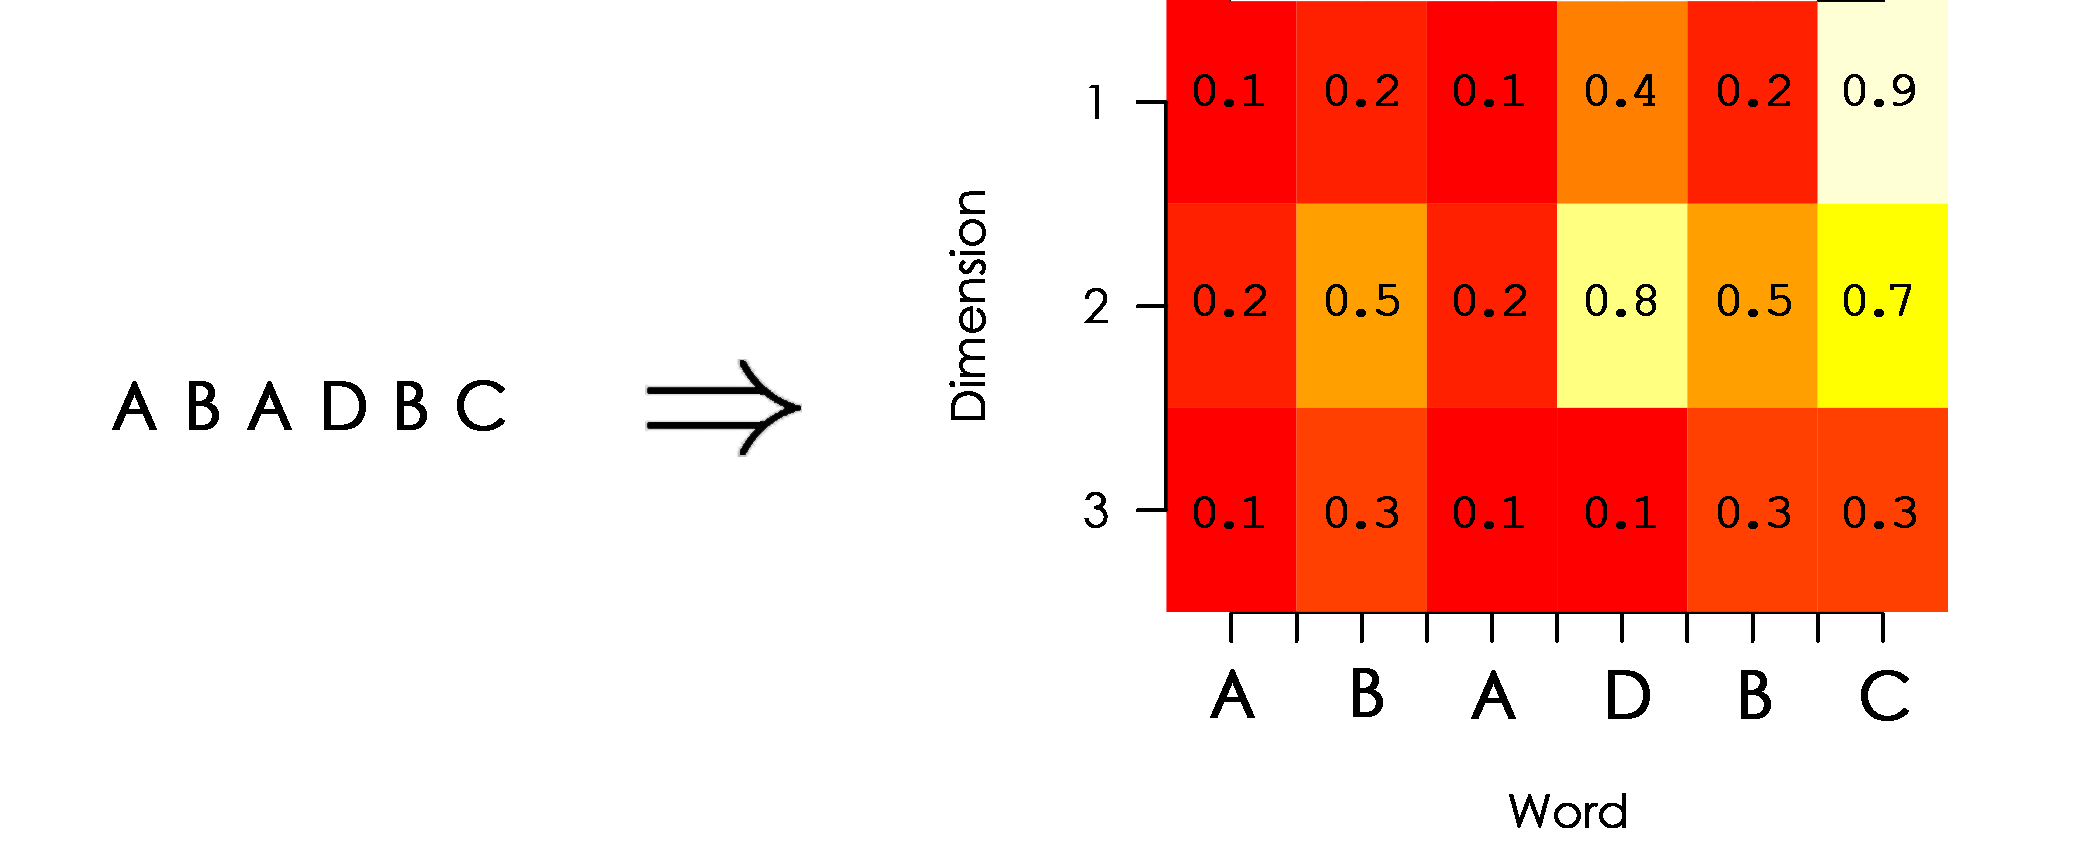
\includegraphics[width=0.7\textwidth]{images/image_classif.png} 
\caption[Example of the text to image procedure.]{Explanation of the mapping 
         between text and image.}
\label{fig:text-classif}
\end{figure}
\end{enumerate}



The images in figure \ref{fig:text-classif-images} were generated from the
introduction of Principia Mathematica by Sir Isaac Newton and Elements of 
Statistical Learning, as well as from Sonnet 18 by William Shakespear. \\

\begin{figure}[!h]
\centering
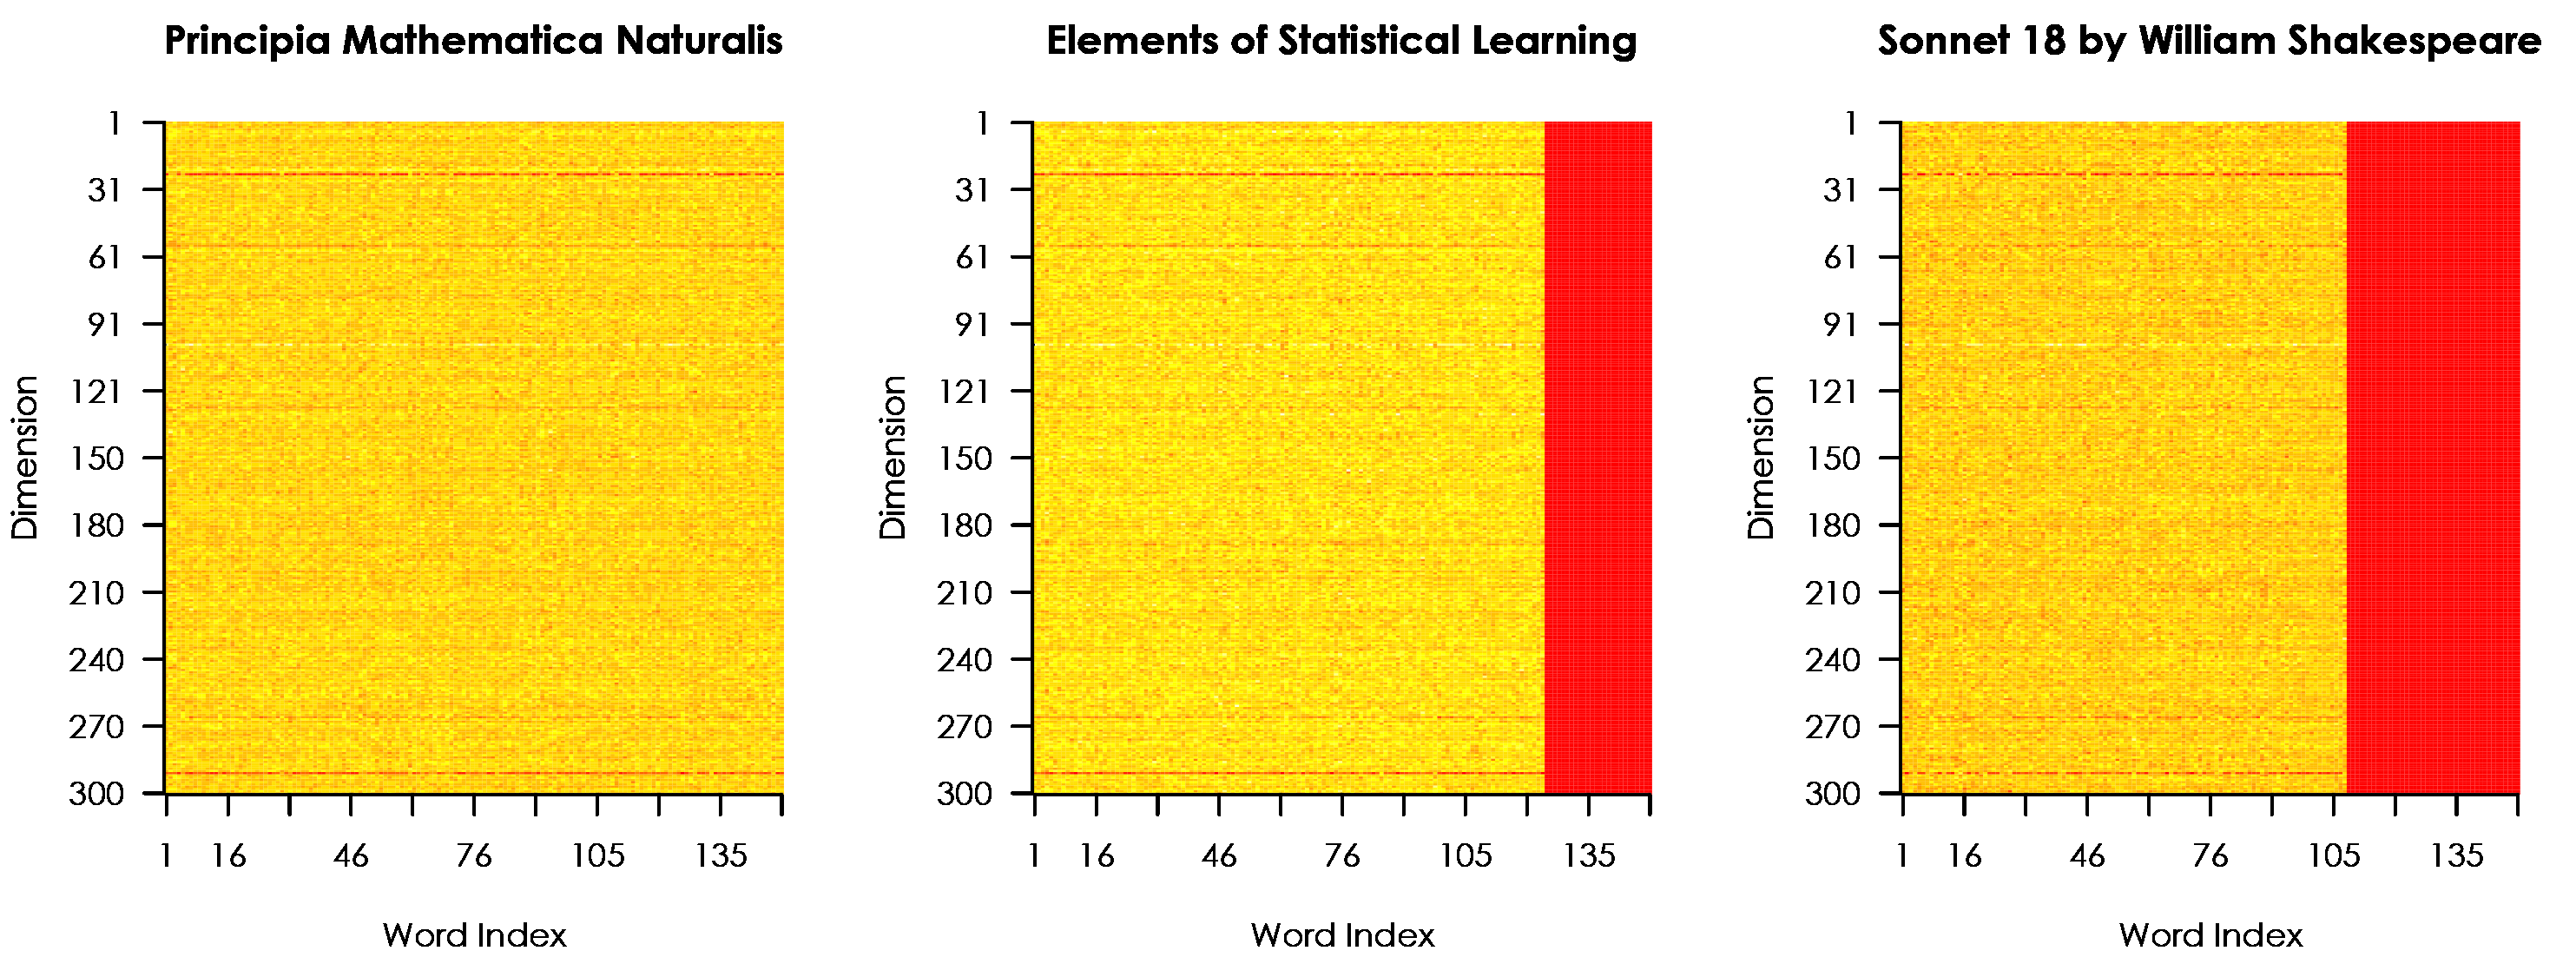
\includegraphics[width=\textwidth]{images/text_images.png} 
\caption[Specific text representation via images.]{Creating images for text using 
         the introduction of Principia Mathematica by Sir Isaac Newton and 
         Elements of Statistical Learning, as well as from Sonnet 18 by William 
         Shakespear. The red bars are missing words filled up to 150 words since 
         image classifier expect a fixed number of pixels.}
\label{fig:text-classif-images}
\end{figure}

The next step would be to run an image classifier (e.~g.~a CNN) on the images
and an label. This classifier could find differences by analysing specific patterns
or maybe the color intensity.

\section{Conclusion}

\begin{itemize}
  \item 
    With GloVe it is possible to create meaningful word embeddings.

  \item 
    \cite{pennington2014glove} compared several models on the word analogy task, 
    whereas GloVe outperforms the others.
  
  \item 
    But accuracy of word analogy task depends not only on the dimension, but 
    also on the corpus.

  \item 
    Use servers or pcs with huge computing power to train GloVe due to 
    the need of huge corpora an computing time!
\end{itemize}